\documentclass[a4paper,english,abstract=on]{scrartcl}

\usepackage{mathtools} % loads amsmath and fixes its bugs in Unicode & XeLaTeX/LuaLaTeX 
\usepackage[english]{babel}
\usepackage[]{unicode-math} % provides Unicode Math support for XeLaTeX/LuaLaTeX 
\usepackage{xcolor}
\usepackage{graphicx}
\usepackage[pdfborder={0 0 0}]{hyperref}
\usepackage[autostyle=true]{csquotes}
\usepackage[backend=biber, style=numeric-comp]{biblatex}
\addbibresource{literatur.bib}
\usepackage{listings}
\lstset{language=SQL}

\title{Exercise 4 Report}
\subtitle{Gruppe 16}
\author{Anastasiia Rubanovych\and Sebastian Funck}
\date{\today}

\begin{document}

\maketitle

\subsection*{a)}
\begin{itemize}
	\item \textbf{Describe in your own words how the program works and how the persistence manager accom-
		plishes logging and recovery.}\\
	
	The persistance manager provides the interface to create transactions that modify an underlying data struture consisting of pages and user data. It is implemented as a Singleton so it has sole control over write and read operations on the respective pages and their content. The main functionality is divided in 3 parts: Handling Transactions, Logging and Recovery.
	
	\item \textbf{Transactions:} The \texttt{PersitenceManager} buffers write operation in a\\ \texttt{ConcurrentHashMap<Integer, PageWrite>} with page-id as key. Comitted transactions aren't persisted right after commit, but rather at a later point when the \texttt{PersitenceManager} decides the buffer has become too large. This can produce the effect of dirty writes, because if Transaction A writes to Page 10, then Transaction B writes to Page 10 and then A commits, the changes aren't persisted, because the change Transaction A to page 10 has been overridden. Only when B is comitted it is eventually written.
	
	\item \textbf{Logging:} Before any operation, the \texttt{PersitenceManager} makes sure the operation is logged and written to the logfile, so that in case a failure occurs, the recovery can recover the system. The operations that are logged are \texttt{write} and \texttt{commit}. \text{begin\_transaction} is not persisted, because we assume that only valid transaction ids make it into the log.
	
	\item \textbf{Recovery:} Because the \texttt{PersitenceManager} is \textit{nosteal} and \textit{noforce} we are doing a redo-recovery. The recovery is done on program start, where the \texttt{PersitenceManager} reads for every page id through the logs and determines winner and loser transactions. Loser transactions are those that don't have an EOT logged. When the winner transactions have been determined the logs of the winner transactions modifying the respective page are replayed starting from the first LSN that is greater than the current Page LSN.
\end{itemize}

\newpage
\subsection*{c.1)}
\begin{itemize}
	\item \textbf{After program completion delete a written page and change the value of a written page. Start the recovery and check if it was successful?}
	\\~\\
	\textit{After first execution:}\\
	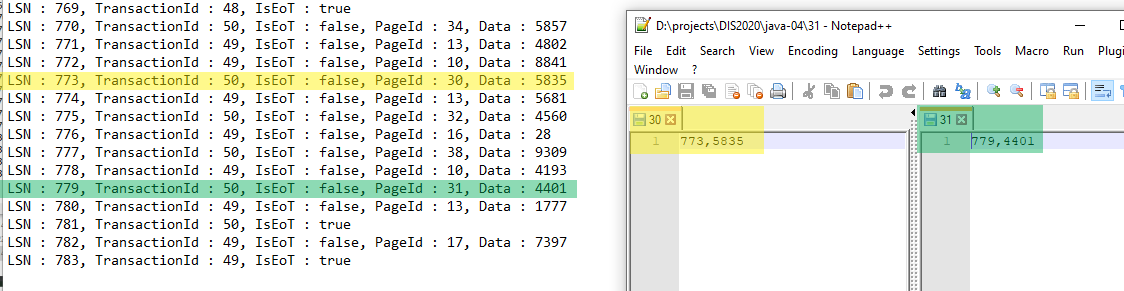
\includegraphics[width=\textwidth,height=\textheight,keepaspectratio]{c1_1.png}\\
	
	\textit{Deleting and modifying the pages:}\\
	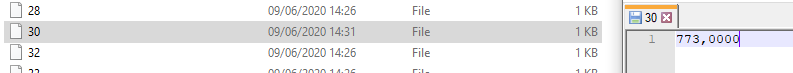
\includegraphics[width=\textwidth,height=\textheight,keepaspectratio]{c1_2.png}\\
	
	\textit{After recovery:}\\
	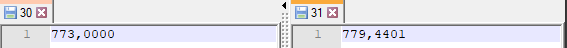
\includegraphics[width=\textwidth,height=\textheight,keepaspectratio]{c1_3.png}\\
	
	The recovery failed for page \texttt{30} because the redo-recovery only checks for writes that satisfy \texttt{LSN(LS) > LSN(Page)}. We were wondering why \texttt{>} is not a \texttt{>=} because this small change would enable us to also recover from that error as well. For page \texttt{31} the recovery worked.
\end{itemize}

\subsection*{c.2)}
	\item \textbf{After program completion find an unwritten change and start the recovery. Was the recovery successful?}
\\~\\
\textit{After first execution:}\\
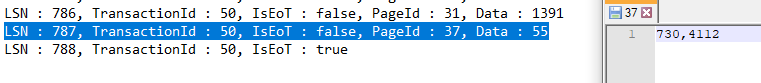
\includegraphics[width=\textwidth,height=\textheight,keepaspectratio]{c2_1.png}\\
\textit{After recovery:}\\
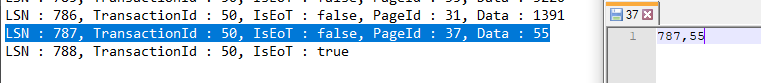
\includegraphics[width=\textwidth,height=\textheight,keepaspectratio]{c2_2.png}\\

The recovery was successful because the value of page 37 corresponds now to the latest comitted log (\texttt{55}).

\subsection*{c.3)}
\item \textbf{After program completion find an unwritten change. Increase the LSN to a value higher than the unwritten change and start the recovery. Was the recovery successful?}
\\~\\
\textit{After first execution:}\\
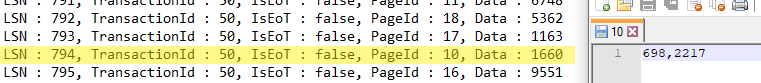
\includegraphics[width=\textwidth,height=\textheight,keepaspectratio]{c3_1.png}\\
\textit{After modification:}\\
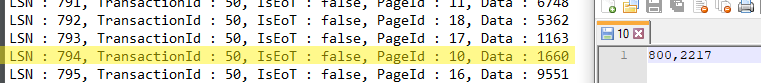
\includegraphics[width=\textwidth,height=\textheight,keepaspectratio]{c3_2.png}\\
\textit{After recovery:}\\
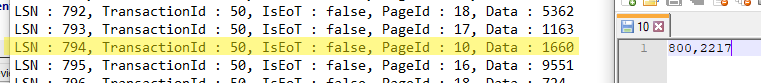
\includegraphics[width=\textwidth,height=\textheight,keepaspectratio]{c3_3.png}\\

The recovery failed, because the redo-recovery assumed the written change is newer than the latest logged write. In theory the recovery could check if this LSN even exists and rollback from there, but this would be an undo-recovery.

\end{document}
